\section{Architectural Description}

\subsection{Overview}
	The logical structure of the service is divided in the following manner:
	\begin{itemize}
		\item{Client Interface Layer:} Its purpose is to interact with all types of users. This includes both a web interface, reserved for customers, and a mobile application,
			used by both customers and drivers.
		\item{Business and Web Layer:} This layer is responsible for the connection of the first layer with the others. It connects users to the information management
			system on the server. This layer operates server-side along with the data management layer. It is also responsible for the management of driver queues and 
			the creation of shared ride orders. 
		\item{Database Management Layer:} This layer is responsible for both user information management as well as reservation storage. Other than saving important and sensitive
			information about the user, it also stores information about the reservations made by users. It communicates with the business layers on a trigger basis when shared rides
			are to be created.
	\end{itemize}
\subsection{High Level Components and Their Interaction}

	\begin{figure}[h!]
		\centering
		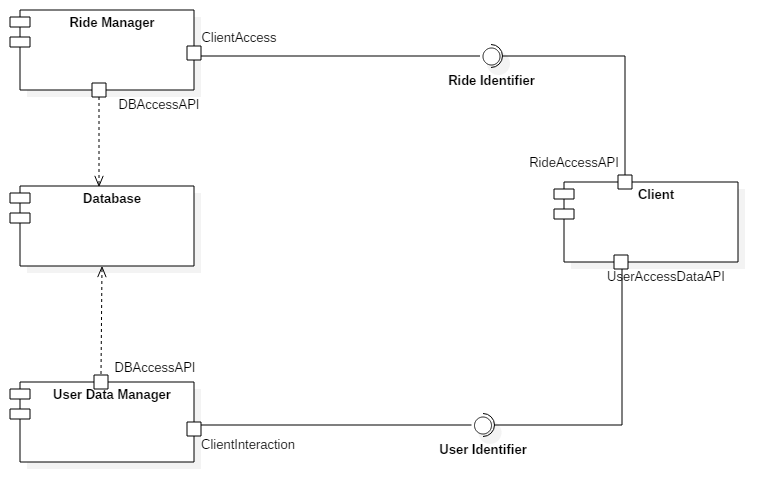
\includegraphics[width=0.9\textwidth]{components/Overview}
	\end{figure}

\subsection{Component View}
	\subsubsection{Client}
		\begin{figure}[h!]
			\centering
			\includegraphics[width=0.9\textwidth]{"components/Client View"}
		\end{figure}
	\subsubsection{Ride Manager}
		\begin{figure}[h!]
			\centering
			\includegraphics[width=0.9\textwidth]{"components/Ride Manager View"}
		\end{figure}
		
	\subsubsection{Data Manager}
		\begin{figure}[h!]
			\centering
			\includegraphics[width=0.9\textwidth]{"components/User Data Manager View"}
		\end{figure}



\subsection{Deployment View}
	\begin{figure}[h!]
			\centering
			\includegraphics[width=0.9\textwidth]{"components/DeploymentDiagram"}
	\end{figure}

\subsection{Runtime View}

\subsection{Component Interfaces}

\subsection{Selected Architectural Styles and Patterns}

\subsection{Further Design Choices}

